\scribe{Ane Santos}



\section{ The hexagonal lattice and laminated lattices}


\subsection{ The hexagonal lattice}

\begin{definition}
Let $v_1,\ldots,v_n\in \ZZ^{d}$  and the lattice $L= _\ZZ\left\langle v_1,\ldots,v_n \right\rangle=\left\{\sum\lambda_i v_i : \lambda_i \in \ZZ\right\}= \left\{M\lambda:\lambda\in \ZZ^{n}\right\}$ with $M=\left[v_1,\ldots,v_n\right]\in\ZZ^{d\times n}$. $M$ is called the \emph{generator matrix} and $\left\langle v_1,\ldots,v_n \right\rangle$ the \emph{integer hull} of the lattice.
\end{definition}


We will study $A_{2,\RR^{2}}$ and $A_{2,\RR^{3}}$.

$A_{2,\RR^{2}}=\left\{\left[\begin{smallmatrix}
1 & 1/2 \\
0 & \sqrt{3}/2 \end{smallmatrix}\right]\lambda:\lambda\in\ZZ^{2}\right\}$, $M=\left[\begin{smallmatrix}
1 & 1/2 \\
0 & \sqrt{3}/2 \end{smallmatrix}\right]$. 

$A_{2,\RR^{3}}=\left\{\left[\begin{smallmatrix}
1 & 0 \\
-1 & 1 \\
0 & -1 \end{smallmatrix}\right]\lambda:\lambda\in\ZZ^{2}\right\}$, $M'=\left\left[\begin{smallmatrix}
1 & 0 \\
-1 & 1 \\
0 & -1 \end{smallmatrix}\right]$. 


We will see both $M$ and $M'$ are generator matrices of the hexagonal lattice.

Firstly, we study $A_{2,\RR^{3}}$:

\begin{figure}[htbp]
\centering
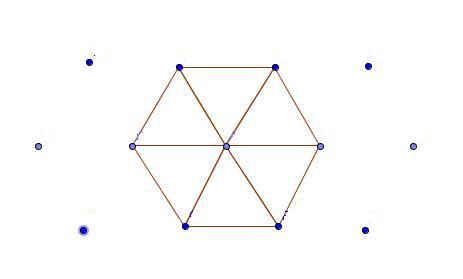
\includegraphics[width=0.5\textwidth]{apunteaklattice}
\caption{$A_{2,\RR^{3}}$}
\end{figure}


\begin{displaymath}
	A_{2,\RR^{3}}=\left\{M'\lambda:\lambda\in\ZZ^{2}\right\}=\left\{\left\begin{bmatrix}
	\lambda_1 \\
	-\lambda_1 + \lambda_2 \\
	-\lambda_2 \end{bmatrix}:\lambda_1,\lambda_2\in\ZZ\right\}
\end{displaymath}

We want to find an hyperplane that contains $A_{2,\RR^{3}}$. We are in $\RR^{3}$, so this hyperplane will be a plane of the form $\left\{x\in\RR^{3}:\left\langle a,x\right\rangle=a_0\right\}$. But we know $0$ is in $A_{2,\RR^{3}}$ so
$H=\left\{x\in\RR^{3}:\left\langle a,x\right\rangle=0\right\}$
$\left\{\omega\in\RR^{3}: \left\langle \omega,x\right\rangle, \forall \in \colospan M\right\}$ where $\colospan M=_\RR\left\langle v_1,\ldots,v_n \right\rangle=im M$ (it is an abelian group and it is also a vector space). So,
$H=\left\{x\in\RR^{3}: \left\langle a,x\right\rangle=0\right\}=\ker M$

$dim \im M=2$ and $dim A_{2,\RR^{3}}=3$ $\Longrightarrow$ $dim A_{2,\RR^{3}}=dim \ker M +dim \im M$ $\Longrightarrow$ $dim \ker M=1$

A generator of $\ker M$ will be $\left(\left[\begin{smallmatrix}
1 \\
1 \\
1 \end{smallmatrix}\right)$

$\left[1 1 1\right]\left[\left[\begin{smallmatrix}
1 & 0 \\
-1 & 1 \\
0 & -1 \end{smallmatrix}\right]=\left[0 0\right]$ $\Rightarrow$ $\ker M= _\RR\left\langle \left[1 1 1\right]\right\rangle$

So $A_{2,\RR^{3}}\subset\left\{x\in\RR^{3}: x_1+x_2+x_3=0\right\}=\left\{x\in\RR^{3}: \mathbbm{1}\right\}$


\begin{definition}
The \emph{Gram matrix} of a lattice $L$ with generator matrix $M$ is $G_L=M^{T}M$.
\end{definition}


\begin{definition}
The \emph{determinant of a lattice} $L$ with generator matrix $M$ is the determinant of the Gram matrix.
$\det L=\det M^{T}\cdot \det M=\left(\det M\right)^{2} $
\end{definition}


\begin{observation}
 $G_L$ is always a symmetric matrix because $G_L^{T}=\left(M^{T}M\right)^{T}=M^{T}M$
\end{observation}


We will see which is the determinant of $A_{2,\RR^{2}}$ and $A_{2,\RR^{3}}$:

$\det A_{2,\RR^{2}}=det \left[\begin{smallmatrix}
1 & 0 \\
1/2 & \sqrt{3}/2 \end{smallmatrix}\right]\cdot\left[\begin{smallmatrix}
1 & 1/2 \\
0 & \sqrt{3}/2 \end{smallmatrix}\right]=\det \left[\begin{smallmatrix}
1 & 1/2 \\
1/2 & 1 \end{smallmatrix}\right]=3/4$

$\det A_{2,\RR^{3}}=\det \left[\begin{smallmatrix}
0 & -1 & 0 \\
0 & 1 & -1\end{smallmatrix}\right]\cdot\left[\begin{smallmatrix}
1 & 0 \\
-1 & 1 \\
0 & -1 \end{smallmatrix}\right]=\det \left[\begin{smallmatrix}
2 & -1 \\
-1 & 2 \end{smallmatrix}\right]=3$


\begin{definition}
The \emph{minimum norm} of a lattice $L$ is $\mu_L=\min\left\{\left\|v\right\|^{2}:v\in L\backslash \left\{0\right\}\right\}$
\end{definition}


The minimum norms of $A_{2,\RR^{2}}$ and $A_{2,\RR^{3}}$ are

$\mu_{A_{2,\RR^{2}}} = 1$

$\mu_{A_{2,\RR^{3}}} = 1$

The determinants and the minimum norms of $A_{2,\RR^{2}}$ and $A_{2,\RR^{3}}$ are different.


\begin{definition}
Two lattices are \emph{isomorphic} if one is obtained from the other by rotation, reflection, translation and sceling.
\end{definition}


We look now to the packing density of $A_{2,\RR^{2}}$ and $A_{2,\RR^{3}}$:

Packing density of L: 

$\Delta_L=\frac{\vol(sphere in packing)}{\vol(\Pi_L)=\sqrt{detL}}$

where $\Pi_L=\left\{\sum\lambda_i v_i : \lambda_i\in\left[0,1\right)\right\}$ is the fundamental parallelpeptide.


In $A_{2,\RR^{2}}$ the radius of the sphere is $\frac{1}{2}$ so the volume is $\left(\frac{1}{2}\right)^{2}\pi$.

$\Delta_{A_{2,\RR^{2}}}=\frac{\left(\frac{1}{2}\right)^{2}\pi}{\sqrt{\frac{3}{4}}}=\frac{\pi}{2\sqrt{3}}$

$\Delta_{A_{2,\RR^{3}}}=\frac{\left(\frac{1}{2}\sqrt{2}\right)^{2}\pi}{\sqrt{3}}=\frac{\pi}{2\sqrt{3}}$

So the lattices are the same.

The most general map between equivalent lattices is $x\longmapsto\alpha A+t$, $t\in\RR^{n}$, $A\in O(n)$, $\alpha\in\RR^{*}$ (the negative are the reflections).

In our case,

$\left[\begin{smallmatrix}
1 & \frac{-1}{\sqrt{3}} \\
-1 & \sqrt{3} \\
0 & \frac{-2}{\sqrt{3}}\end{smallmatrix}\right]\left[\begin{smallmatrix}
1 & \frac{1}{2} \\
0 & \frac{\sqrt{3}}{2}\end{smallmatrix}\right]=\left[\begin{smallmatrix}
1 & 0 \\
-1 & 1 \\
0 & 1\end{smallmatrix}\right]$

So, we have two different ways to write the same lattice. The advantages of $M'$ over $M$ are that the coordinates are nicer and the symmetries of the lattice are more easily seen.


\begin{claim}
Any permutation of the coordinate axes in $\RR^{3}$ is a symmetry of $A_{2,\RR^{3}}$.
\end{claim}


\begin{proof}
Let $P:\RR^{2}\longmapsto\RR^{3}$ be a symmetry, i.e. $P(L)=L\Rightarrow\forall x\in L, P(x)\in L \Rightarrow\forall\lambda\in\ZZ^{2}, \exists\beta\in\ZZ^{2}:PM\lambda=M\beta$ ($x=M\lambda$).

We want to proof that, if $P$ is a permutation then $\forall\lambda\in\ZZ^{2}$ we can find a $\beta$ where this is true.
We know $P$, $M$ and $\lambda$, so we have to find $\beta$. This is a linear equation for $\beta$.
We must show that the linear equation $M\beta=b$ has a unique solution for any $b_\lambda =PM\lambda$.
The solution is unique if $\rank M$ is maximal, i.e. $\rank M=2$.
$M$ has rank 2 so we only have to see if it always has a solution.
For the fundamental theorem of linear algebra part 2 the system has a solution $\Longleftrightarrow$ $b\in \colspan M=\im M$ $\Longleftrightarrow$ $b\bot\left(\colspan M\right)^{\bot} $ $\Longleftrightarrow$ $b^{T}y=0$ whenever $y\bot \colspan M$ $\Longleftrightarrow$ $b^{T}y=0$ whenever $y^{T}M=0$

Let $\left[0 0\right]=\left[y_1 y_2 y_3\right]\left[\begin{smallmatrix}
1 & 0 \\
-1 & 1 \\
0 & -1\end{smallmatrix}\right]=\left[y_1 - y_2, y_2 - y_3\right]$

$y^{T}M=0$ $\Longleftrightarrow$ $y=\alpha\mathbbm{1}$
$b^{T}y=\lambda^{T}M^{T}P^{T}\alpha\mathbbm{1}=\alpha\lambda^{T}M^{T}P^{T}\mathbbm{1}=\alpha\lambda^{T}M^{T}\mathbbm{1}=0$
$M^{T}\mathbbm{1}=0$ because $\mathbbm{1}$ is in the $\ker$ of $M$.
\end{proof}


\subsection{Laminated lattices}


Define $\mathbb{L}_0=\left\{L^{0}\right\}$, $L^{0}=\left\{0\right\}=\mathbb{R}^{0}$ the zero dimensional lattice and $m:=4$ (usually $m$ is 4 because the sphere has radius 1).

For $n>>0$, $\mathbb{L}_{n+1}=\left\{L_1^{n+1},\ldots,L_{a_n}^{n+1}\right\}$ is the collection of $n+1$-dimensional lattices such that
\begin{enumerate}
\item each $L_i^{n+1}$ has constant minimal norm $m$
\item each $L_i^{n+1}$ contains at least ones $L_j^n$ as a sublattice
\item each $L_i^{n+1}$ has minimal determinant subject to (1), (2)
\end{enumerate}


We will see which are this lattices:

\begin{enumerate}
\item $\mathbb{L}_1$ : $k\ZZ$

It needs minimal norm m=4 $\Rightarrow$ $2\ZZ$ 
It satisfies (2) and (3).
So the unique laminates lattice of rank 1 is $2\ZZ$.


\item $\mathbb{L}_2$ :

$M=\left[\begin{smallmatrix}
2 & 0 \\
0 & 2\end{smallmatrix}\right]$ 

Satisfies (1),(2) and (3). It is $2\ZZ^{2}$.


We don't need to use integer points, it only needs to contain $2\ZZ$.

We have two candidates:  $2\ZZ^{2}$ and $A^{2}$. We will see which of them is what we need:

$\det 2\ZZ^{2}=\det M^{T}M=\det\left[\begin{smallmatrix}
4 & 0 \\
0 & 4 \end{smallmatrix}\right]=16$ where $M=\left[\begin{smallmatrix}
4 & 0 \\
0 & 4 \end{smallmatrix}\right]$.

$\det A^{2}=\detM^{T}M=\det\left[\begin{smallmatrix}
4 & 2 \\
2 & 4 \end{smallmatrix}\right]=12$ where $M=\left[\begin{smallmatrix}
2 & 1 \\
0 & \sqrt{3} \end{smallmatrix}\right]$.


$\det A_2 < \det 2\ZZ^{2}$

The area of the parallelpeptide is less than the square. So $\mathbb{L}_2$ will be $A_2$.
\end{enumerate}
We will see now how can we do the sphere packing:

\begin{figure}[htbp]
\centering
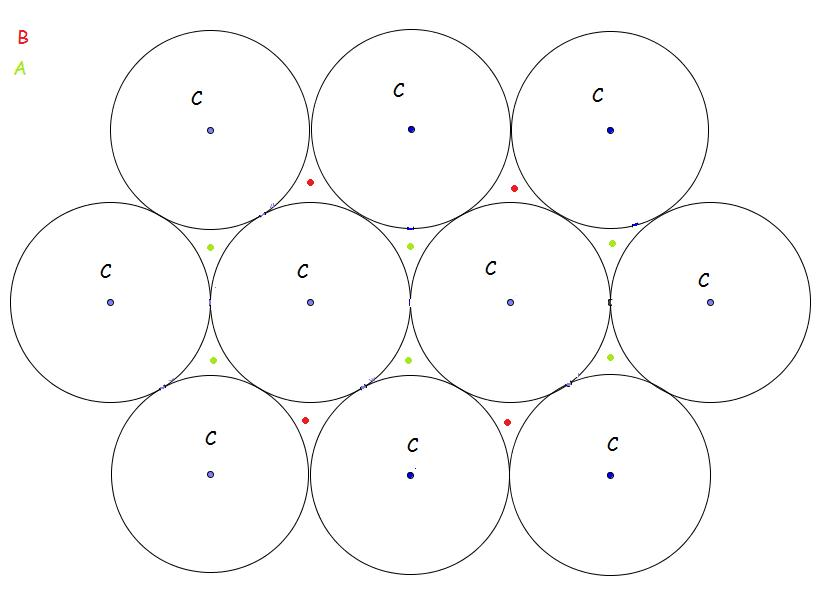
\includegraphics[width=0.5\textwidth]{apunteslattice}
\caption{sphere packing}
\end{figure}

For the next layer we have two options, put them (the centers of the sphere) over the deep holes A or over the deep holes B. For the second layer we put, we will have the possibility of putting them over C (the centers of the spheres of the first layer).
Each lattice obtained by snugly packing copies of $A_2$ is determied by the sequences
ABAB.... (this is the hexagonal close packing(He attoms))
ABCABC....(this is the face-centered cubic lattice ($A_3$))
of equivalence classes of deep holes.

In each step there are two options to choose from, which makes uncountable many possibilities in total.


